%%%%%%%%%%%%%%%%%%%%%%%%  Denoising.tex 04/08/2012  %%%%%%%%%%%%%%%%%%%%%%%%%%
%%                                                                          %%
%%                                                                          %%
%%%%%%%%%%                                                       %%%%%%%%%%%%%
%%%%%%%%%%    More information: see the header of IEEEtran.cls   %%%%%%%%%%%%%
%%%%%%%%%%                                                       %%%%%%%%%%%%%
%%%%%%%%%%%%%%%%%%%%%%%%%%%%%%%%%%%%%%%%%%%%%%%%%%%%%%%%%%%%%%%%%%%%%%%%%%%%%%


\documentclass[10pt,conference,letterpaper,doublecolumn]{IEEEtran}



\usepackage[dvips]{color}
\usepackage{epsf}
\usepackage{times}
\usepackage{epsfig}
\usepackage{graphicx}
\usepackage{url}
\usepackage{amsmath}
\usepackage{amssymb}
\usepackage{amsxtra}
\usepackage{algorithm}
\usepackage{algorithmicx}
\usepackage{algpseudocode}


\usepackage{cite}
\usepackage{listings}
\usepackage{verbatim}
\usepackage{pseudocode}
\usepackage{indentfirst}
\usepackage{float}
\usepackage{fancyhdr}
\pagestyle{fancy}
\rhead{CS263C Animats-Based Modeling}
\makeatletter
\newcommand{\rmnum}[1]{\romannumeral #1}
\newcommand{\Rmnum}[1]{\expandafter\@slowromancap\romannumeral #1@}
\makeatother

\newtheorem{condition}{Condition}
\newtheorem{assumption}{Assumption}
\newtheorem{colloary}{Colloary}
\newtheorem{theorem}{\bf Theorem}
\newtheorem{proposition}{Proposition}
\newtheorem{lemma}{Lemma}
\newtheorem{example}{Example}
\newtheorem{notation}{Notation}
\newtheorem{definition}{\bf Definition}
\newtheorem{remark}{Remark}
\linespread{1.0}
%\textfloatsep=3pt plus 3pt
\dbltextfloatsep=3pt plus 3pt

%%%%%%%%%%%%%%%%%%%%%%%%%%%%%%%%%%%%%%%%%%%%%%%%%%%%%%%%%%%%%%%%%%%%%%%%%%%%
% Some variables

\newcommand{\SIR}{{\xi}}
\newcommand{\SF}{{L}}
\newcommand{\sis}{\sigma^2}
\newcommand{\betas}{{\left(1+\beta^{2} \right)}}
\newcommand{\BS}{{\mathrm{BS}}}
\newcommand{\plcnst}{{\kappa}}        % path loss constant
\newcommand{\plexp}{{\mu}}            % path loss exponent
\newcommand{\shadow}{{\zeta}}             % shadowing rv
\newcommand{\sigmaS}{\sigma_{\mathrm{S}}} % shadowing standard deviation
\newcommand{\Kpole}{K_{\mathrm{pole}}}



% ------------------------------------------------------------------
% -- ADJUST THE PAGE SETUP


\begin{document}
\title{Evolution of Predator Avoidance and Alarm Calls}
%\subtitle{test}
%\author{Guanya Yang (204378262), Fan Li (304414453)}

\author{Guanya Yang(\tt{guayang@ucla.edu}) \\
        ID: 204378262
      \and
        Fan Li(\tt{fanli.cs.ucla@gmail.com}) \\
        ID: 304414453
      %\and 
      %Guanya Yang(\tt{guayang@ucla.edu}) \\
      %  ID: 204378262
        }
\date{}
\maketitle



\begin{abstract}
We implemented a predator-prey system in which prey animats escaped from predator animats while foraging for food in a 2D environment. The design of the animat brains include neural networks and reinforcement learning. Our results demonstrated prey learning in three stages: 1) learning how to avoid two types of predators 2) learning how to avoid a new type of predator 3) learning how to emit alarm calls while foraging for food in groups.
\end{abstract}

\section{Introduction}
In natural ecosystems, food webs are composed to multiple organisms on different trophic levels. Animals in the middle levels consume organisms in lower levels while escaping from predators in higher levels. We focus on prairie voles, a primary consumer whose main predators include hawks, foxes, and snakes. Prairie voles live in colonies, which we simulate in the situation of group foraging \cite{animal1, animal2}.
\subsection{Hypothesis}
Given prey vole animats that must forage for nuts and avoid three types of predators to survive, they learn how to avoid the different types of predators while maintaining sufficient energy levels. After the voles adapted to the predators, we introduced the condition that the voles cannot sense prey while they are eating. Then they must also learn to respond to alarm calls from fellow voles in order to continue to evade predators. Over time, we hypothesize that the fitness of the prey animats would increase as they became skilled at evading predators.
\subsection{Goals}
\begin{enumerate}
\item Phase \uppercase\expandafter{\romannumeral1}: The prey vole learns how to avoid two types of predators, the hawk and the fox. \\
\item Phase \uppercase\expandafter{\romannumeral2}: A new snake predator is introduced, which the vole will have to learn how to avoid in addition to the hawk and the fox. \\
\item Phase \uppercase\expandafter{\romannumeral3}: Now, when the voles are eating nuts, they cannot sense predators at the same time. Thus, they have to find food in a group and any voles that are not eating learn to send warning signals to their fellow voles.
\end{enumerate}
\section{Implementation}
\subsection{Environment and Physics}
We designed simple animats, specifically a pack of 30 prey animats and 3 predator animats, in a 2D world. Prey animats can sense both their own kind and the predators. All 3 predators can also sense the prey. We will not distinguish genders nor age among the animats. \\

The 2D world also includes various holes, bushes, trees, and nuts. To make it easier to observe interactions in our environment, we decided to make the total number of nuts present simultaneously to be 60; whenever the number of nuts drops below 60, we automatically replace it with another one placed in a random location on the screen.
\subsection{Methodology}
We concentrate of a lower level of animat complexity and a higher level of learning and adaptability. The specific abstractions used are: 
\begin{enumerate}
\item Voles must eat nuts to survive, as measured by a hunger meter that decreases with time. 
\item Voles die on contact from predators or when their hunger meter goes to zero. (For Phase \uppercase\expandafter{\romannumeral2}, to give the prey opportunities to learn how to escape from the snake, we set the probability of a snake eating the prey upon contact to be 50\%) 
\item Each type of animat will generate a specific signal. All other animats are able to sense the signal and infer the signal type, strength, and direction within a given radius.
\item The prey moves slower than the predator because the prey’s brain is more advanced than that of the predator. All predators move at the same speed. 
\item Animats do not mate or reproduce, but we artificially change the population size in our experiments. 
\item The bodies of animats physically take up space but are allowed overlap with other each other, as well as with shelter.
\end{enumerate}

\section{Animat Design}
\subsection{Predator}
There are three types of predators as follows: 
\begin{enumerate}
\item Hawk: voles can evade the hawk by burrowing under a hole or hiding under a bush
\item Fox: voles can evade the fox by burrowing in a hole or climbing up a tree
\item Snake: voles can evade the snake by climbing up a tree or hiding under a bush, but there’s a 50\% chance of the snake catching the prey under a bush.
\end{enumerate}

We implemented a Feedforward Neural Networks (FFN) as the controller. We chose an FFN as the brain controller for predator to make the predator smart enough to catch prey but not so smart as to wipe out the prey population. The FFN for predators is designed as follows:

\begin{enumerate}
\item Input Layer: Linear layer of size 6
\item Hidden Layer: Sigmoid layer of size 6 
\item Output Layer: Linear layer of size 5 
\end{enumerate}

According to Hornik et. al., the sizes of the input layer and output layer should correspond to the size of the sensors and effectors of the brain~\cite{FFN}. Since there are 5 different actions to take (one for each direction of movement and one for predating), we set the output layers to 5. For the input layer, we could use as little as 3 inputs to represent all the parameters from the predator's sensors: two for the x- and y-coordinates of sensed prey and one for the hunger meter. Normalizing each parameter, they can cover all possible inputs. During our supervised learning process, we found that the FFN converges faster if we specified the inputs more concretely by increasing input layer of a size 6. Since the size of the hidden layer should be be between the size of the input and output and a sigmoid function offers greater number of outputs, we implement the hidden layer as a sigmoid layer of size 6 to include as many hidden states as possible~\cite{FFN2}.\\

After the construction of the neural network, we designed the parameters. We generated a set of sample data to train the predator and a supervised learning process to set all the parameters in the network. With this FFN, once the predator is able to sense any prey animats in a given range and its own hunger level, it can decide on the shortest path to pursue the prey.

\subsection{Prey}
The brain is a Recurrent Neural Network (RNN) implemented with Q-learning, a type of RNN. We chose to use Q-learning to clearly implement reinforcement learning.
\subsubsection{State Representations}
The sensors for the prey are used to generate a representation of the state it is currently in. However, in addition to the perceptions of the prey, we include a variable that indicates whether or not the predator sensor was activated in the past 5 consecutive time steps. We represented our states as a 4-tuple $(L, F, P, R)$ where $L$ represents the location which indicates whether or not the prey is around the corner of the map with two different values, $F$ represents the sense of food with two different values, $P$ represents the exist of predators and their types with $8$ different values for all $3$ types of predators and $R$ represents whether predators have recently appeared. Thus, we have an entire state space with $2 \times 2 \times 8 \times 2$ combinations of the percepts, which is $64$ unique states in total for Phase \uppercase\expandafter{\romannumeral1} and Phase \uppercase\expandafter{\romannumeral2}. 
For Phase \uppercase\expandafter{\romannumeral3}, there is another sensor for the alarm calls and represented by two different values. However, the alarm sensor is active only if the predator sensor is disabled since voles that are eating cannot sense the predators and would need to avoid them by sensing alarm calls. Thus there are $2 \times 2 \times 2 \times 2$ which is $16$ different states added.

\subsubsection{Actions}
There are five different effectors of the prey animat: $Up, Down, Left, Right, Stay, Eat$ and $Call$ additionally for Phase \uppercase\expandafter{\romannumeral3}. The prey should be capable of foraging for food or avoiding predators with only these five simple actions.

% \subsubsection{Actions}
% As we found out that with more specific states, the animat is more smart, we thought it could be true that it will help if we define actions as meaningful skills like foraging food or escaping from predator. This is what we tried at first and it actually works but soon we find the point is that we are actually equipment our preys with given powerful skills like knowing what is foraging food and what is running away from predators. This leads to contradictions with our assumptions because we want our prey to learn to be smart. Then we realized that the only actions our prey can take should be the functions of its effectors. Thus the actions of prey are defined as $Up, Down, Left, Right, Stay, Eat$ and $Vole$ additionally for Phase \uppercase\expandafter{\romannumeral3}. This is quite inspiring because when the prey is finally work, it means that it is capable to act a function of foraging food or escaping the predators with only known the simple actions listed above. Moreover, this looks like the prey is smart enough to know that in order to escape, it has to take two $Up$ actions and then three $Left$ actions to a shelter and several $Stay$ actions to wait the predator to leave.

\subsubsection{Rewards} \label{Rewards and Discussions}
The core of the entire Q-learning algorithm is based on the premise of a reward scheme~\cite{qlearn}. In order for Q-learning to function correctly, it is imperative that the prey be able to determine the approximate value of an action immediately after performing the action. A simple reward scheme for our problem could be a positive reward after eating food or getting close to food; a positive reward when staying in or getting close to a shelter when chasing by a predator; a negative reward when getting close to a predator and so on. However, since the situation is quite complicated with finding food and escaping from at least two kinds of predators with different shelters, this simple solution will not work well so we introduce additional terms for reward. We define a value function for the prey as follows:
\begin{equation} \label{V}
V = \alpha * E + \beta * S + \gamma * F
\end{equation}
where $\alpha, \beta$ and $\gamma$ are the weight coefficients of $E$, $S$, and $F$.

$E$ is the estimate of possible space that the prey could travel to, with two special cases. The first case is when the prey is around the corner (Fig.~\ref{space1}). The prey should prefer not to go to the corner since it is neither good place to find food nor a safe place to escape from predators. This is important as the environment is bounded so the actions the preys take when it is in the middle of the environment between when it is around the corner can be quite different.
\begin{figure}[H]
  \centering
  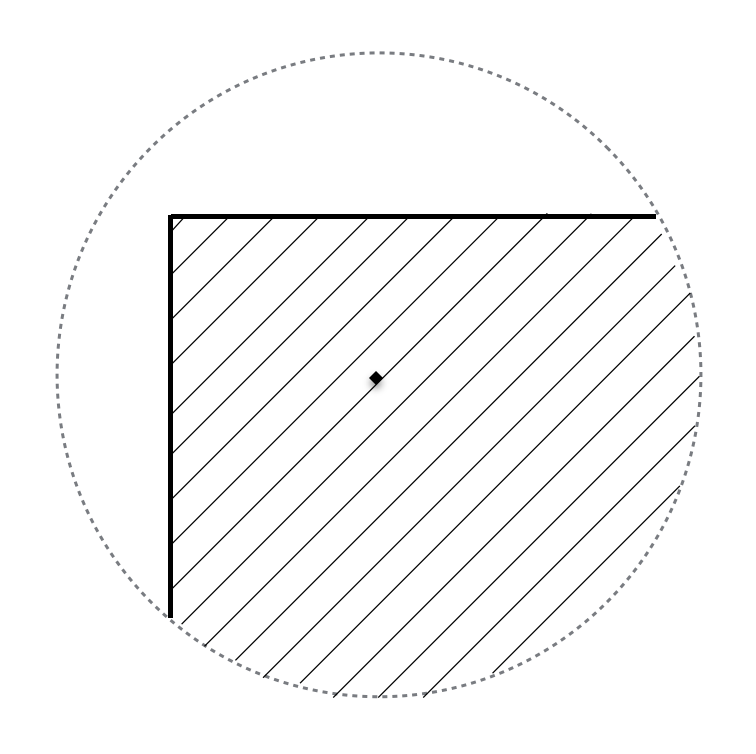
\includegraphics[scale=0.4]{space1.png} \\
  \caption{The case when the prey is around the corner. The solid lines represent the boundaries of the environment and the circle represent the sense range of the prey. The shaded area is the estimation of possible space that the prey could go to around the corner.}
  \label{space1}
\end{figure}
The estimation of $E$ also indicates the distance between the prey and the predators. As shown in Fig.~\ref{space2}, the possible space is divided by the median line between the prey and the predator in this case. The estimation space to travel decreases as the distance from predators decreases. We use the estimation space because we found out that in order to escape while several predators exist in different positions, the best strategy is to move to the places where the prey can take the greatest number of possible actions. In general, using this estimation instead of the distance between the prey and the predator allows the prey to calculate more precisely the reward for situations when it is around the corner of the environments and when predators appear in different positions. 
\begin{figure}[H]
  \centering
  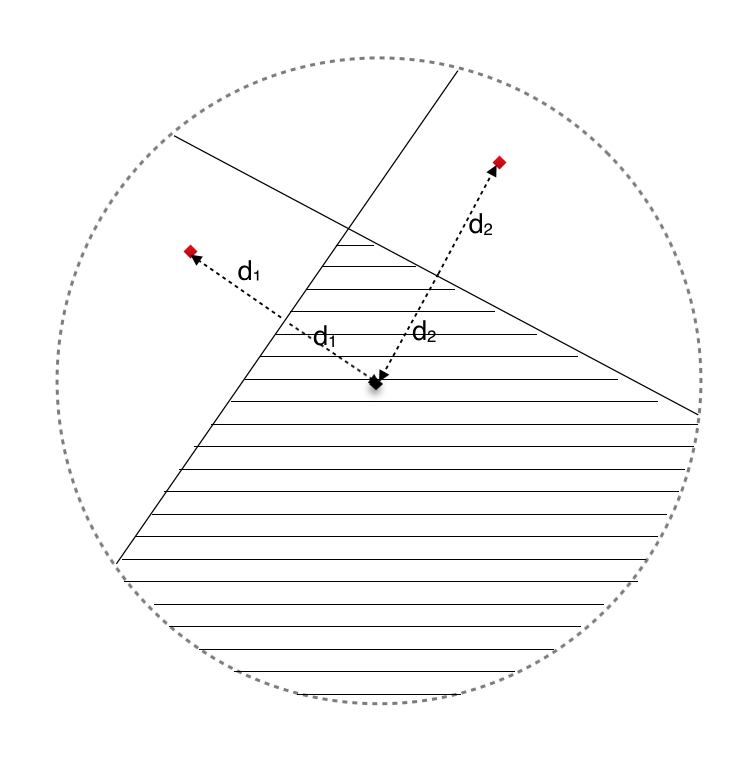
\includegraphics[scale=0.4]{space2.png} \\
  \caption{The case when the predators exist. Predators are represented by red points and the solid lines is the median line between the predators and prey. The shaded area is the estimation of possible space that the prey could go to around the corner. }
  \label{space2}
\end{figure}
$S$ incdicates whether the prey should escape to shelter to avoid any predators sensed and is defined as:
\begin{equation}
S = \sum_{s \text{sensed}, i} p^i_s*\left| p^i \right|
\end{equation}
where $\left| p^i \right|$ is the amount of predator with type-$i$ sensed and the value $p^i_s$ represent whether $s$ is a correct shelter for predator $p^i$. In Phase \uppercase\expandafter{\romannumeral1}, the prey is engineered with knowing the correct shelter for hawks and foxes and in  Phase \uppercase\expandafter{\romannumeral2} the prey does not know the coefficient $p^3_s, \forall s$. We introduced a reinforcement process to change the coefficient as long as it is attacked by the snake. \\

The food function $F$ in Eqn. 3 describes the distance between the prey and the food, which is defined as:
\begin{equation}
F = \max_{f\in S} \frac{1}{Dis(prey, f)}
\end{equation}

We only estimate the food whose coordinates is within the range of the possible space that the prey can travel to that is also away from any sensed predators. \\

In summary, our reward is a combination of the varying value function representing the combination of the prey’s distance from predators, shelter, and food. With the appropriate weights for each part of the equation, the prey is able to consider and decide on the appropriate action to take given a combination of factors from the its surroundings.
\subsubsection{Evolution}
For Phase \uppercase\expandafter{\romannumeral3}, we originally intended for the prey to somehow learn to forage for food in groups if they are unable sense predators while eating. However, under our given design of the states and actions of the prey animat, it is not possible to let them learn how to forage in groups since there is no such behavior to reward them for foraging in groups in the first place. We needed to engineer the group foraging behavior and then let the voles adapt to prefer the group foraging behavior to the original solitary foraging behavior. To demonstrate such an adaptation, we modeled an evolutionary process instead of relying solely on reinforcement learning. During the evolution process, we generated a mutation of our prey at the beginning of the experiment with the recessive genotype $aa$; the initial population contained the homozygous dominant genotypes $AA$. We chose the mutation to be recessive because we did not want the voles to adapt to group foraging too quickly, making the problem too easy. The prey with the mutated recessive genotype would have knowledge of forging food in a group of two and is stimulated by an additional positive reward. Upon reaching food, we randomly one of the voles to eat and the other to warn its companion if appears within its sense range.

\section{Problems Encountered}
In the beginning, we contemplated whether to implement a simple design of actions as moving in either four directions, staying in one place, or eating, or to implement a more abstract design of actions representing an overall goal, such as foraging for food or escaping from a predator. Although the animat learned more quickly when we implemented the abstract design, we realized that this contradicted our hypothesis because this was merely a form of supervised learning. In order to stay true to our plan of reinforcement learning, we ended up choosing the actions to be simple, letting the animats learn how to pursue complicated goals by taking a set of simple actions. \\

Designing the predators to find food was relatively straight-forward, but adding the additional goal of escaping from a generic type of predator was much more difficult. For example, the prey do not have memory of where it traveled or what it encountered before, so it would try to move towards the predator once the predator was out of its sense range. We solved this problem by adding internal states to specify what the prey has sensed. We also tried a lot effort in coming up with a good estimation of the reward function to make the prey more capable in learning different kinds of skills. \\

Another issue was that the animat would move back and forth in one spot and seem to forget how to find food. Eventually, we discovered the cause was due to how we set up the possible actions for each state to take. For example, we define each state to randomly choose an action with probability $p_a$. Each state will converge to an action if there is one action with a large enough $p_{a'}$ to dominate all other possible actions. However, we had set several states such that there was a great chance of choose between two actions (i.e. moving up or left if it sensed a predator in the upper left quadrant), making it impossible for each state to converge to one action. Since a state can lead to any other state in the Q-table, the non-convergence of one state will also lead to the non-convergence of the other states, which prevents learning from finishing. We solved this issue by a deeper examination of all the states that the prey may encounter and the transformation probability between completely different states and handle them with carefully designed reward function.

\section{Experimental Results}
\subsection{Visualized Simulator}
We implemented a visualized simulator for a better understanding and testing whether our animats are acting in the way we desire. Fig.~\ref{env} shows a simulator with the size $800\times 600$. The simulator is used for testing whether our algorithm is working or not, however, it is not a good way to show the results when dozens of animats added. Thus, we carried out other experiments for different phases.

\begin{figure}[H]
  \centering
  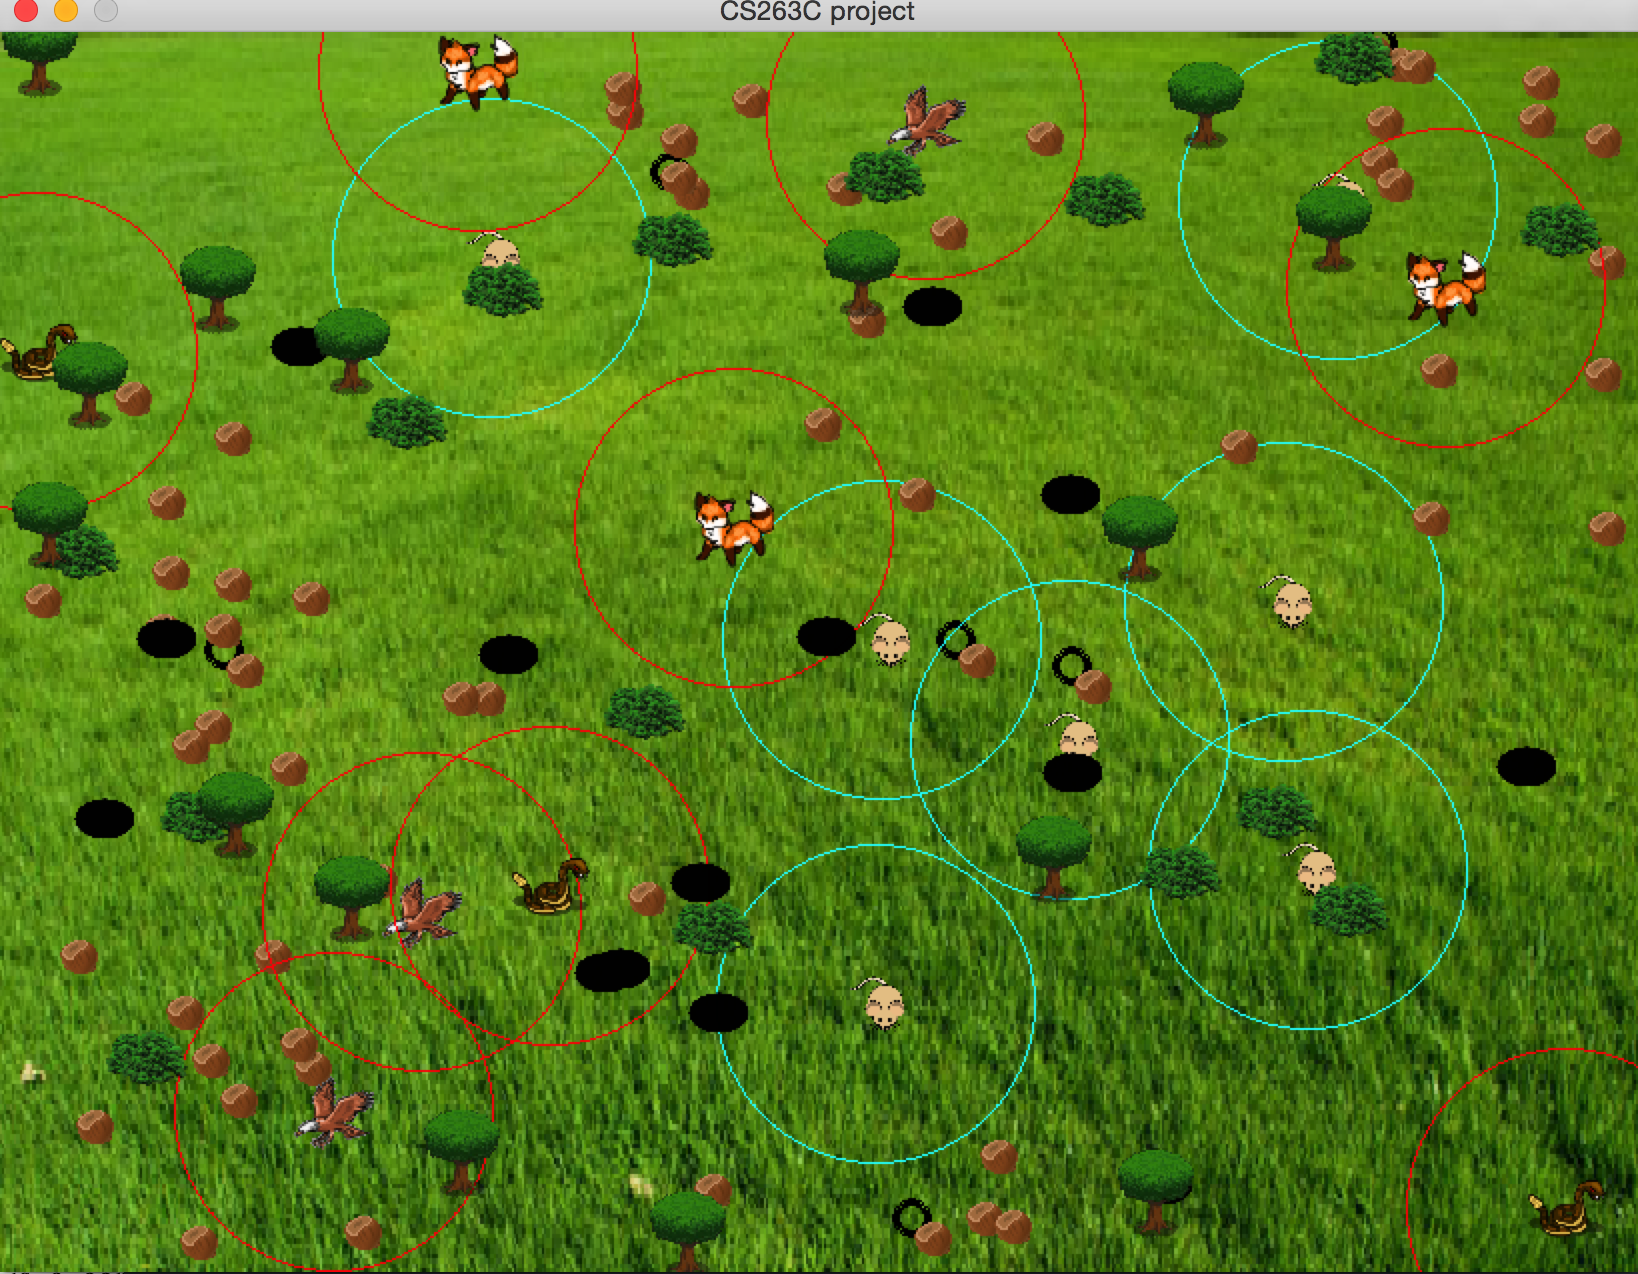
\includegraphics[scale=0.3]{simulator.png} \\
  \caption{A visualization simulator for our environment: animals in red circles are predators, while animals in blue circles are prey; circles represent their sense ranges. Nuts and three types of shelters are randomly distributed throughout the environment.}
  \label{env}
\end{figure}

\subsection{Phase \uppercase\expandafter{\romannumeral1}}
The experiment parameters are set as follows:
\begin{table}[H] 
\centering 
\begin{tabular}{|c|c|c|c|}
\hline
\text{Parameter}&  \text{Food} & \text{Predator} & \text{Shelter}\\
\hline
\text{Value} & 40 & $3$ \text{(Hawk and Fox)}  & $15$ \text{(Each)}\\
\hline
\end{tabular}
\end{table}

We determined the carrying capacity of the environment with the above given parameters by initially creating a population of 300 voles. The result is shown in Fig.~\ref{test}. Over time, as the number of nuts is held constant, the voles compete for food while their hunger levels decrease. Since all voles start with the same initial hunger level, a majority of them die from hunger at the same time of around 475 ticks. Immediately afterwards, the population stabilizes to around 30 voles. Thus, we decided to set our initial population for the three phases to 30 voles. Any further changes in the population can then be assumed to be solely due to predation.
\begin{figure}[H]
  \centering
  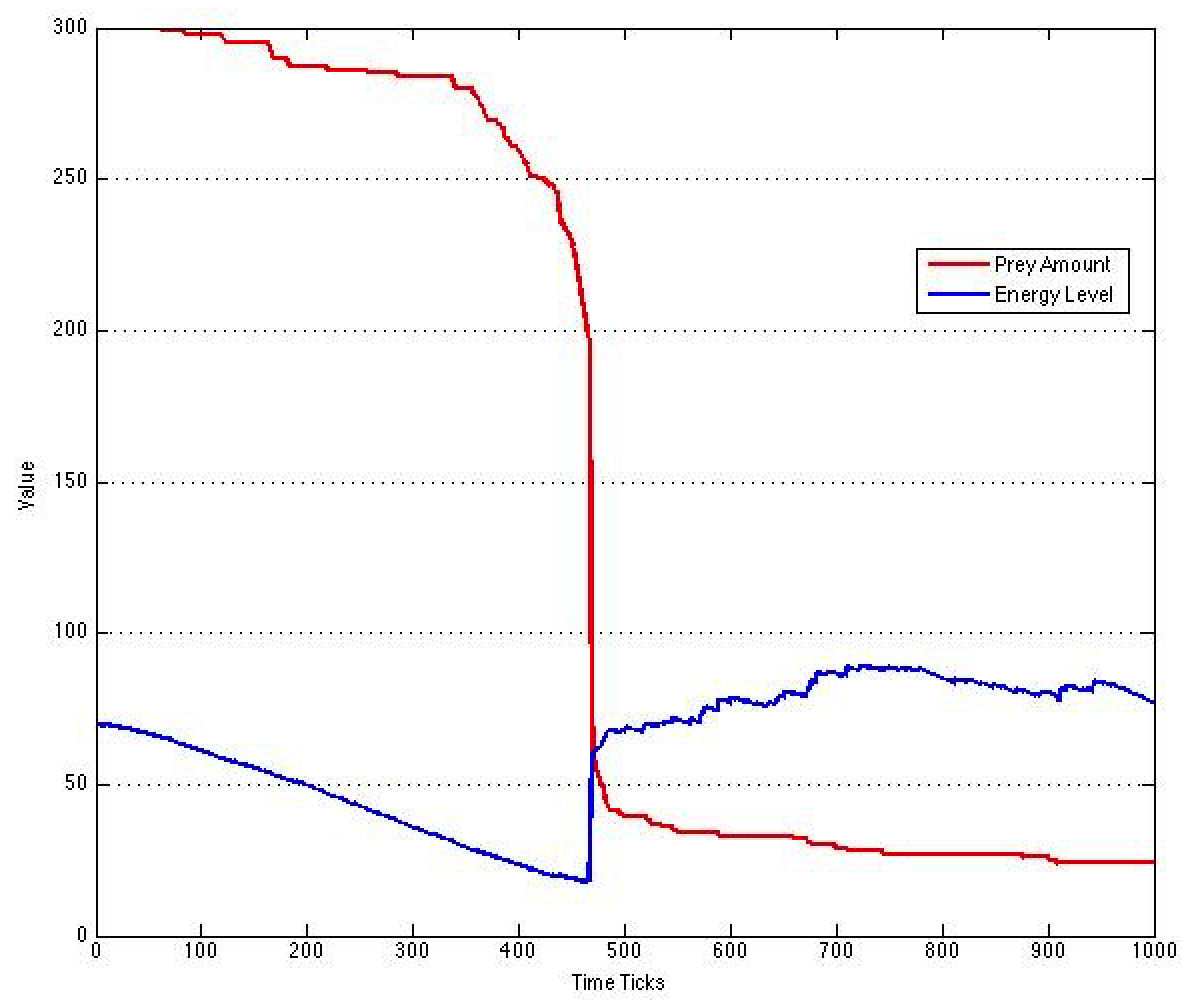
\includegraphics[scale=0.35]{parameter_test.png} \\
  \caption{The carrying capacity of the environment for 40 nuts is around 30 voles. All voles were initially placed in the environment with the same hunger level. At around 475 ticks, there is a steep decline in the population as many voles die from hunger, right before the population stabilizes.}
  \label{test}
\end{figure}

Without adding any new prey to the environment, the population steadily decreases over time due to predation (Fig.~\ref{without}). However, the population never reaches 0 even after 1000 ticks, indicating that the voles were able to successfully learn how to evade the first two predators, the fox and the hawk.
\begin{figure}[H]
  \centering
  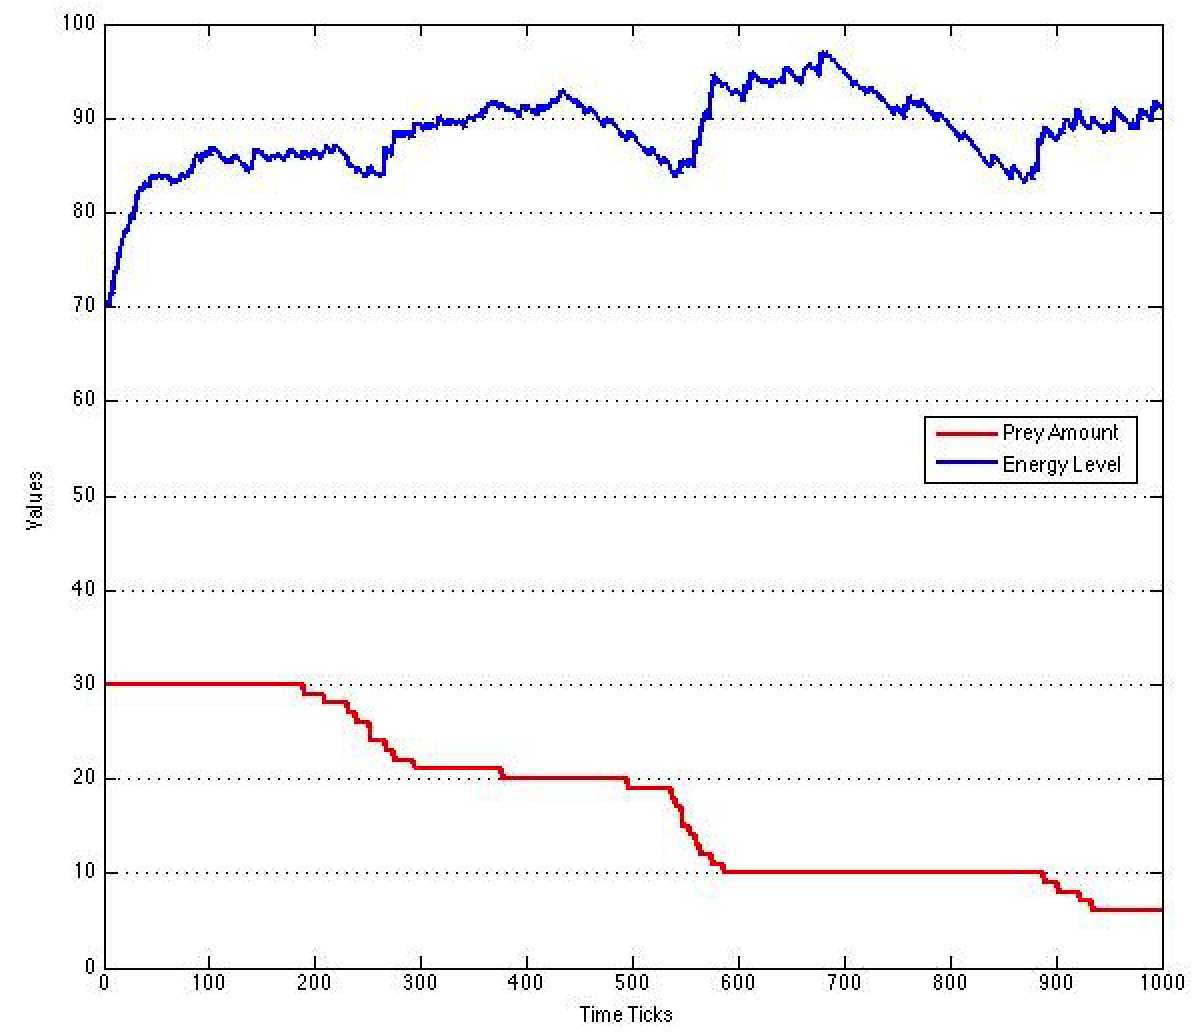
\includegraphics[scale=0.35]{without_mating.png} \\
  \caption{A population of 30 voles without any artificial reproduction in a 2-predatory environment results in a steady decline in population over time.}
  \label{without}
\end{figure}
To determine the parameters for artificial reproduction of voles in an environment with predators, we tested different rates of reproduction at each time tick (Fig.~\ref{with}). We define the rate of reproduction as the chance of a vole mating with another vole and producing one offspring at each time tick. imitating sexual reproduction whereby two voles mate to produce one surviving offspring. Although real voles tend to have much litters of 5 to 10 each year, we limited the litter to only one offspring since there isn't enough predation in our simulation to control such a high reproduction rate [1]. Eventually, we found that a mating rate of $0.005$ imitates natural prey population fluctuations and sustains our vole population in the presence of the initial two predators.

\begin{figure}[H]
  \centering
  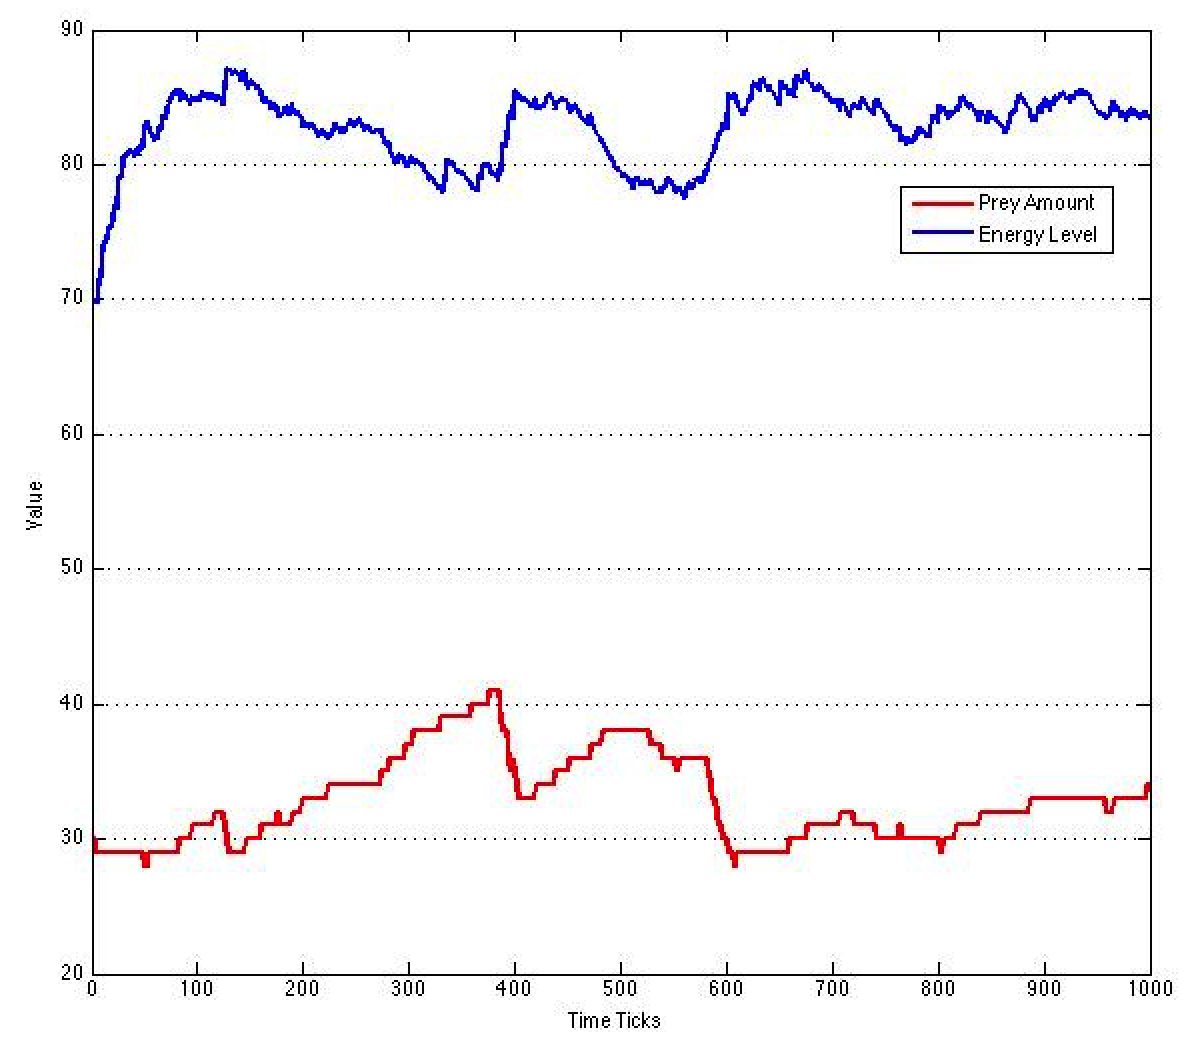
\includegraphics[scale=0.35]{with_mating.png} \\
  \caption{After introducing artificial reproduction at a rate of $0.005$ in a 2-predatory environment, the vole population stays relatively constant around 30. (The environment capacity)}
  \label{with}
\end{figure}

\subsection{Phase \uppercase\expandafter{\romannumeral2}}

We now introduce a new predator, the snake, into the environment and the experimental results are shown in Fig.~\ref{p2}.

\begin{figure}[H]
  \centering
  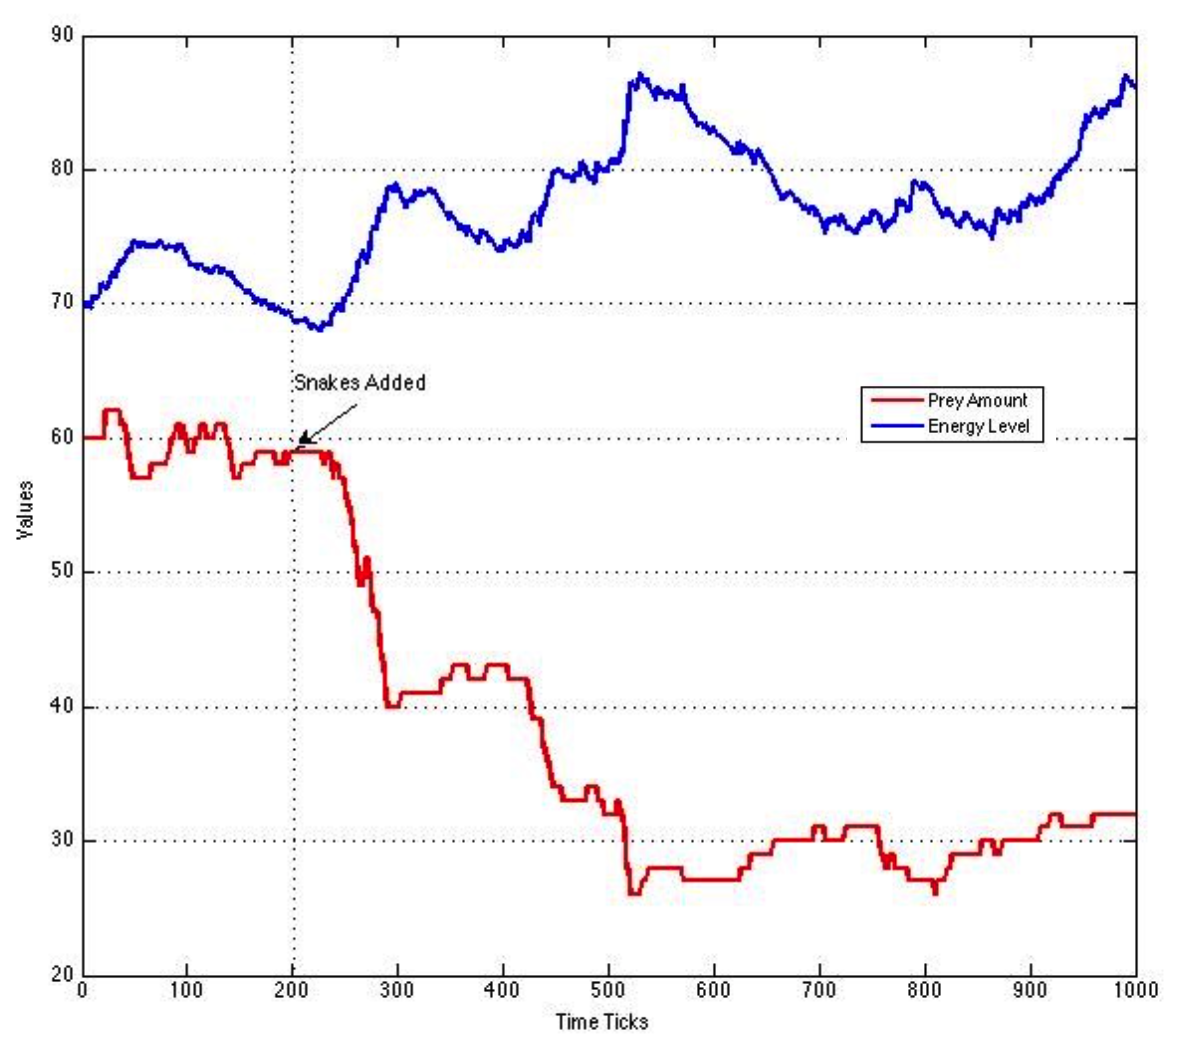
\includegraphics[scale=0.35]{phase2.png} \\
  \caption{After introducing the new snake predator at $200$ ticks, the vole population initially steadily decreased, eventually reaching a stable size of around $30$ at $500$ ticks.}
  \label{p2}
\end{figure}
 Although the voles can sense that the snake is a dangerous predator, they do not know which type of shelter to choose to escape to. By trial-and-error and reinforcement learning, the voles eventually learn to choose the bush and the hole, with a preference for the hole. For the experiment, we set the Food Amount to be 60 and increase the initial number of preys to 60 because many of them will die before they learn to avoid the snake. The slope of population decrease is large initially as the voles have not yet learned which shelter to escape to. As the voles learn successfully over time, the slope becomes less steep. There is even a slight increase in population after 800 ticks, which shows how the voles are beginning to flourish just a couple hundred of ticks after the appearance of a new predator.\\
 
 Next, we examined the relative positions of the prey animats compared to the locations of the shelters dispersed in the environment. An assortment of the three types of shelters were randomly distributed throughout the environment (Fig.~\ref{map}).
\begin{figure}[H]
  \centering
  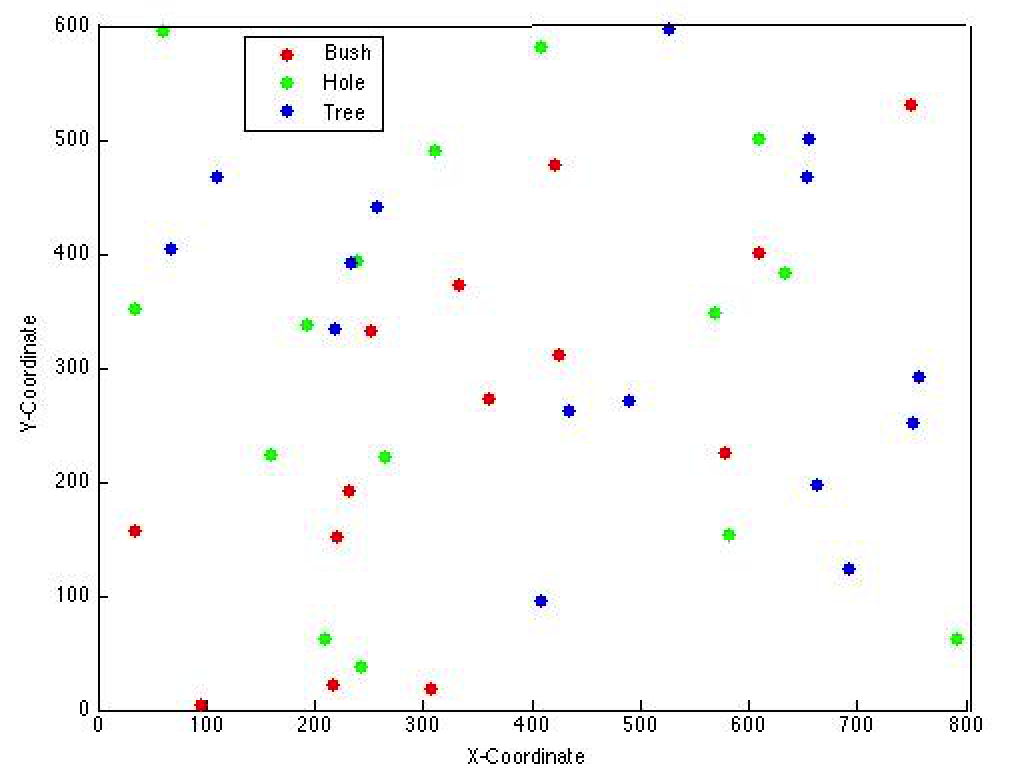
\includegraphics[scale=0.4]{map.png} \\
  \caption{The map of shelters in the Phase \uppercase\expandafter{\romannumeral2} experiment.}
  \label{map}
\end{figure}
\begin{figure}[H]
  \centering
  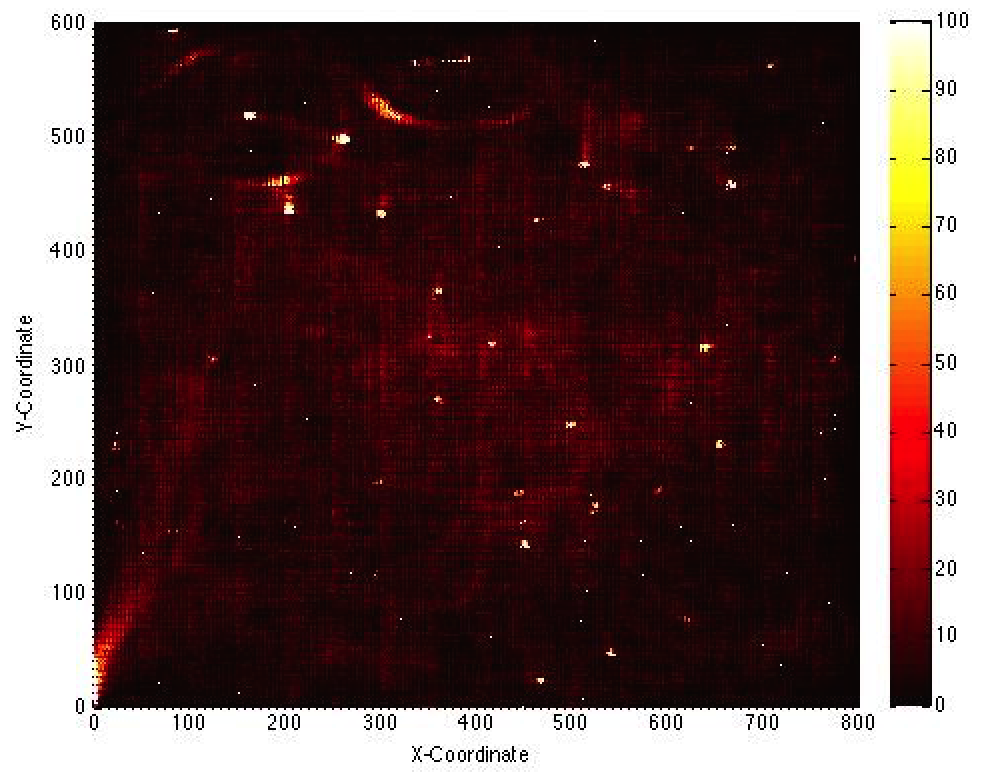
\includegraphics[scale=0.45]{map_rate.png} \\
  \caption{The heat map of locations the prey animats visited. Yellow indicates locations visited most frequently while black indicates locations visited least frequently.}
  \label{mapr}
\end{figure}
 As expected, the locations the animats visited (Fig.~\ref{mapr}) roughly corresponded to the locations of the shelters as they tended to move to those areas to escape from predators. Other red areas most likely correspond to nut positions. One aspect of the result we weren’t expecting was the high frequency that the animats were visiting the lower left corner. Even though we attempted to prevent the voles from moving towards corners in our experimental setup, our approach was not foolproof. It is possible that a vole may have moved to a corner to eat a nut, but also begins to sense a predator, which may be able to corner the prey and capture it.


\subsection{Phase \uppercase\expandafter{\romannumeral3}}
We initially created a population of voles that composed of 0.9 expressing the native phenotype and 0.1 expressing the recessive gene for group foraging. Over time, as is shown in Fig.~\ref{p3}, the voles that did not exhibit the group foraging gene died off and failed to reproduce, while those that were recessive for the gene flourished, eventually making up almost 100 percent of the final population at 5000 ticks. The voles that participated in group foraging exhibited greater fitness by adapting to the handicap of being unable to sense predators while eating.

\begin{figure}[H]
  \centering
  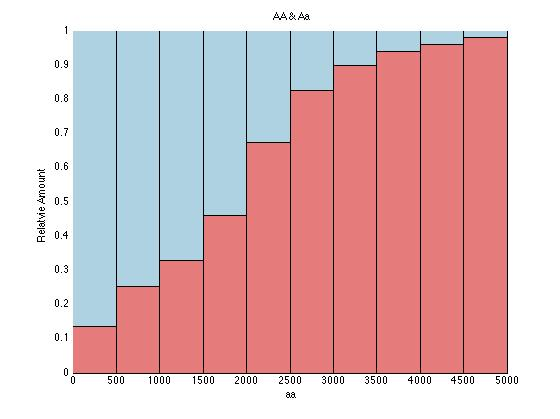
\includegraphics[scale=0.45]{phase3.jpg} \\
  \caption{The relative population of voles with the dominant (Red) and recessive (Blue) phenotypes for the group foraging gene. The amount is the average taken over every 500 ticks}
  \label{p3}
\end{figure}

Fig.~\ref{p32} shows the energy level and prey amount after $4000$ ticks in experiment for Phase \uppercase\expandafter{\romannumeral3}.
\begin{figure}[H]
  \centering
  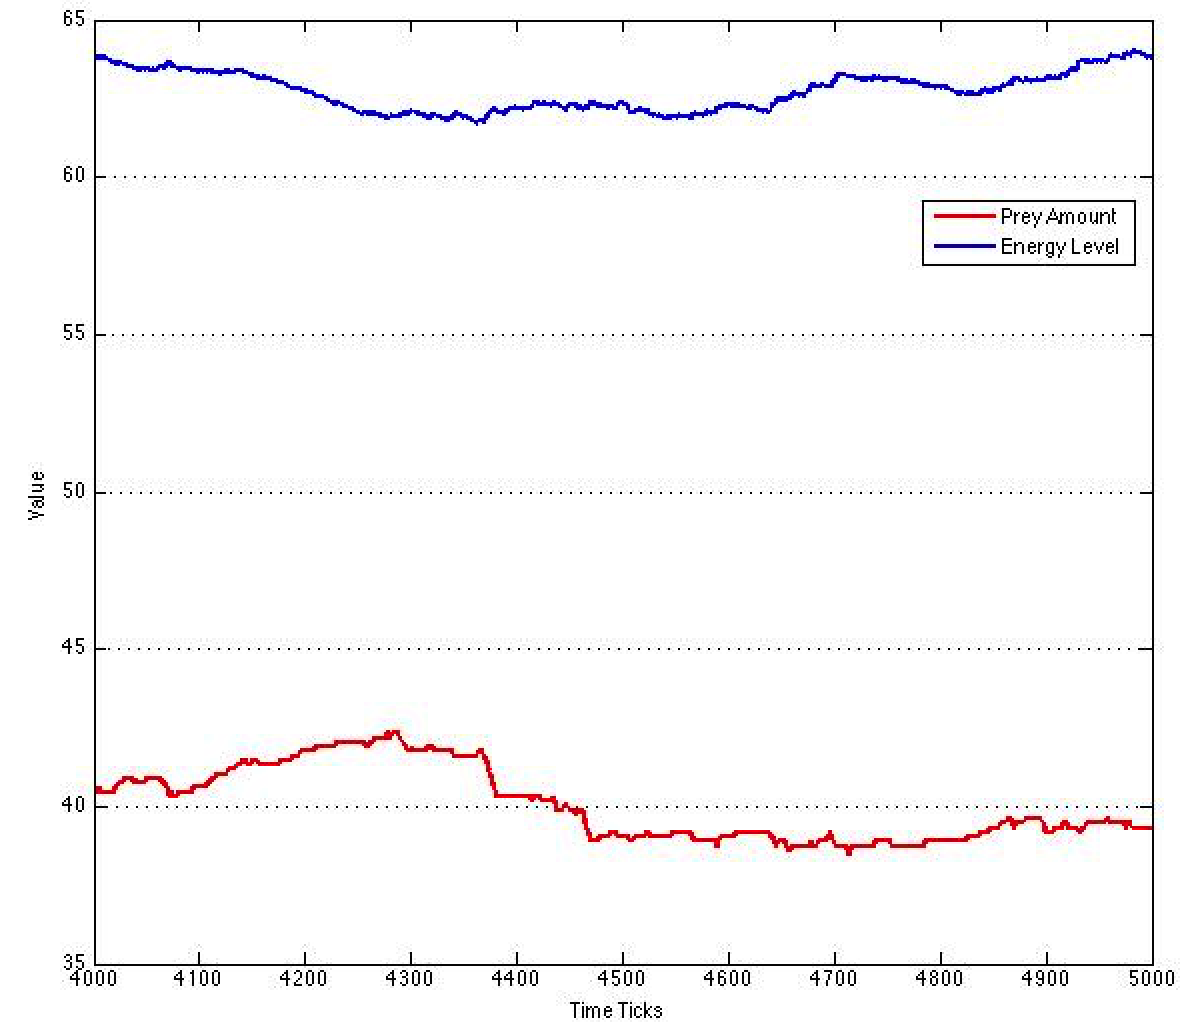
\includegraphics[scale=0.35]{p3.png} \\
  \caption{The energy level and prey population stays relatively constant throughout the whole time period of Phase \uppercase\expandafter{\romannumeral3}.}
  \label{p32}
\end{figure}
Compared to an environment with only two predators in Fig.~\ref{with}, environment with three predators results in lower average energy but higher survival rate. The lower average energy is likely due to the increased complexity of foraging for food in groups. Conversely, the higher survival rate suggests that the prey have learned to better escape from their predators by working together. By evoking an alarm call to warn their neighbors, the voles effectively increase each other’s sense range by sharing the information within all of their sense ranges.
\section{Current Status and Future Directions}
Currently our Q-learning prey animats are able to successfully escape from three types of FFN predator animats by escaping to appropriate types of shelter, while foraging for nuts to survive. Through reinforcement learning, the voles utilize the information they sense from the environment to decide on the best action to take at each time tick; over time, we can regard the summation of set of simple individual actions as broad, abstract goals.

If we had more time, we would have liked to explore Phase III more, using strictly reinforcement learning to let the prey animats adapt to group foraging, without relying on evolution. This would entail adding more states and actions to the design of the prey animat to support group foraging behaviors. 

It would also be interesting to further investigate how the prey animats would adapt to smarter predator animats that are also implemented with Q-learning, to group hunting with more than two prey animats at a time, or to other more complex environmental situations. These experiments would more closely mimic predator-prey interactions in nature. We hope that our results contribute to a greater understanding of animal group hunting and to the field of animat research.


\section{Language/Tools/Packages:} 
\begin{enumerate}
\item Language: \emph{Python}
\item FFN network using \emph{PyBrain} \\
\underline{www.pybrain.org}
\item Visualized simulation based on \emph{Pygame} \\
\underline{www.pygame.org}
\end{enumerate}


\section{Contributions}
Both authors contributed equally to the project, from the coding and implementation to the presentation and written report.
%\begin{equation}
%F = \sum_{f \text{sensed}} \frac{1}{Dis(prey, f)}
%\end{equation}
% E =  \alpha * A \\
% S =  \beta \sum_{s \in S} p_s * \frac{1}{Dis(prey, s)} \\
% F = \sum_{f \in F} \frac{\beta}{Dis(prey, f)}
% \end{equation}

% \section{Related Work}%2
% Some contextual multi-armed methods can be applied to this problem, but they are relatively slow as we must find out every co-efficient between new user's information and historical user data. To simplify the computational complexity, some researchers use the similarity to reduce the burden of exploitation. 

% We refer recent recommendation techniques that tackle both making dynamic exploration / exploitation (bandit algorithm) and considering the user’s situation in recommendation$^{[1]}$. To improve exploitation of the $\epsilon$-greedy algorithm, the Decreasing-$\epsilon$ –Greedy algorithm extends it with setting out the optimal trade-off value  which is iteratively updated in the method. The algorithm uses a set of weights $w=\{ w_1,w_2, ... , w_t \}$ to keep track of the feedback of each $\epsilon_i$, and $w_i$ is increased if receiving a number of positive feedbacks when user uses $epsilon_i $. This algorithm takes  the user’s situation into account and balances the exploration and exploitation tradeoff in a dynamic way. However, each time we still have to update the parameters and make comparisons to find the best $\epsilon_i$. The time complexity of this algorithm is $O(n^2)$.

% Compared to traditional contextual multi-armed method, using the similarity properties between contexts can greatly reduce the computational complexity. Clustering is another feasible way to help us build the recommendation system.

% \section{Problem Statement and System Model}
% In our system, we want to give some new users some recommendations about music genre, but they do not tell us what exactly music type they are into. But we have some personal informations of these users, and these informations are basically their age, gender, hobbies, and other preferences that can reflect some aspects of their characters.   To implement the recommendation process, we will take advantage of 400 previous user's data. Those data contains complete personal profiles and their music tendencies, which can serve as a reference to our work. 

% We consider each user's whole data as a tuple item $x_i(x_i^1, x_i^2, ... , x_i^n)$, and with the use of clusters, we connect users that has similar information and music preference together. The main idea of our model is that we find the most related cluster to the new user and use the item information in this cluster to recommend the music genre. Euclidean Norm($||x_i-x_j||$) is used to quantify how close two items are. To make this searching action faster, we build a search tree to realize quick search. Each node of the tree represents different size of clusters. 

% % \begin{figure}[H]
% %   \centering
% %   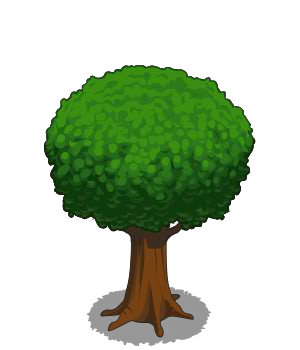
\includegraphics[scale=0.6]{tree.png} \\
% %   \caption{Item-Cluster Tree $^{[2]}$ }
% % \end{figure}
% A parent node cluster contains all their children node clusters. The deeper a node is, the smaller the cluster size is. 
% Every time a recommendation is provided, the online user will decide whether he likes the recommended music type. The accuracy of the recommendation is the reward we get.

% This recommendation process can also combine with reinforcement learning. Every time we make an  accurate recommendation, we would append this new item into the cluster we use to do the prediction. Along with new user arrives, this learning can be more stable and pertinent. 

% \section{System Diagram}
% \subsection{Item-Cluster Tree}
% Figure 2 illustrates the way how the Item-Cluster tree is built. $L$ denotes the depth of the tree. The layer $i$, where $i \in {0,1,2,...,L-1}$, represents each node and leaf. For  all the centering items in layer $i=L-1$, they are the leaf items.

% % \begin{figure}[h]
% %   \centering
% %   \includegraphics[scale=0.45]{system_diagram1.png} \\
% %   \caption{System Diagram: Item-Cluster Tree}
% % \end{figure}

% \subsection{Recommendation Action}
% When each new user arrives, we firstly find the closest cluster at the top of the tree. Then we find the most related children cluster corresponding to the previous parent cluster. We repeat this action until we find the closest cluster at the bottom layer of the tree(leaf layer). So after the search, every user in this final cluster and the new user may have very similar personal information and music preferences. Based on this final cluster, we can do some recommendations. The whole process is shown in Figure 3.

% % \begin{figure}[h]
% %   \centering
% %   \includegraphics[scale=0.6]{system_diagram2.png} \\
% %   \caption{System Diagram: Recommendation Action}
% % \end{figure}
 
% \subsection{Proposed Algorithm}
% The algorithm consists of two major parts, just as showed in part A and part B of Section \uppercase\expandafter{\romannumeral4}. First, we build up the Item-Cluster tree with the use of current history users' data. Then each time when we get a new user's personal information or other hobbies and preferences, we will search for the most related history users to get necessary data for our information.
% %
% %\begin{algorithm}
% %\caption{self-learning algorithm of adjusting regulation time interval}
% %\begin{algorithmic}
% %\For {each time interval $\alpha$}
% %\State calculate average ACE of time period $\alpha$; 
% %\If {$ACE > \epsilon$}
% %\State $\alpha \rightarrow \alpha\cdot e^{-k_1(ACE-\epsilon)}$;
% %
% %\Else
% %\State $\alpha \rightarrow \alpha\cdot e^{-k_2(\epsilon - ACE)}$;
% %\EndIf
% %\EndFor
% %\end{algorithmic}
% %\end{algorithm}
% \section{numeric results}
% The computational Complexity of the first part of our method in this music recommendation system is $O(n\log n)$. Since this process is completed offline, so we do not care about this part. What we do focus is the recommendation action, which is an online action. With the help of searching tree from root to leaf, we could find the most related cluster item with a cost of $\log n$ complexity. So our expected result is that our algorithm performs faster than the conventional Multi-Bandit UCB Algorithm or other traversal algorithms, which have complexity of approximately $O(n^2)$.
% \section{conclusion}
% The process of Item-Cluster tree buildup is offline, so we saved a lot of time and computational complexity. The recommendation action could be diverse, as we can use average method or add new user's data to the tree, and etc. to get the recommendation data. In the future, we can implement this method into real webpage or ios/Android application to test the feasibility of our algorithm.  



\bibliographystyle{IEEE}
\begin{thebibliography}{10}

\bibitem{animal1} Solomon, Nancy G., and Joseph J. Jacquot. ``Characteristics of resident and wandering prairie voles, Microtus ochrogaster." \textit{Canadian Journal of Zoology}, 80.5 (2002): 951-955.
\bibitem{animal2} Lowell L. Getz, Betty McGuire, Theresa Pizzuto, Joycde E. Hofmann, Barbara Frase. Social Organization of the Prairie Vole (Microtus ochrogaster). \textit{Journal of Mammalogy}, Vol. 74, No. 1, 1993, pp. 44-58.
\bibitem{FFN} Kurt Hornik, Maxwell Stinchcombe, Halbert White. Multilayer feedforward networks are universal approximators, \textit{Neural Networks}, Vol. 2, Issue 5, 1989, pp. 359-366, ISSN 0893-6080, http://dx.doi.org/10.1016/0893-6080(89)90020-8.
\bibitem{FFN2} Anil K. Jain, Jianchang Mao, K.M. Mohiuddin. Artificial Neural Networks: A Tutorial, \textit{Computer}, Vol. 29, no. 3, pp. 31-44, March, 1996
\bibitem{qlearn} Dini, Steve, and Mark Serrano. ``Combining Q-Learning with Artificial Neural Networks in an Adaptive Light Seeking Robot." (2012).

% \bibitem{textbook} L. Song, C. Tekin, and M. van der Schaar, ``Online Learning in Large-scale Contextual Recommender Systems," accepted and to appear in 
% \textit{IEEE Transactions on Services Computing}.
\end{thebibliography} 

\end{document} 